\documentclass[conference]{IEEEtran}
\IEEEoverridecommandlockouts
% Template version as of 6/27/2024

\usepackage{cite}
\usepackage{algorithmic}
\usepackage{graphicx}
\usepackage{textcomp}
\usepackage{xcolor}
\usepackage{amsmath,amsxtra,amssymb,amsthm,latexsym,amscd,amsfonts}
\usepackage[utf8]{vietnam}
\usepackage[english]{babel}
\usepackage{fancyhdr}
\usepackage{multirow}
\usepackage{booktabs} % Để kẻ bảng đẹp hơn
\usepackage{url}

\pagestyle{fancy}
\renewcommand{\headrulewidth}{0pt}
\renewcommand{\footrulewidth}{0pt}
\renewcommand{\sectionmark}[1]{\markright{\MakeUppercase{#1}}{}}

% Điều chỉnh lề theo template FJCAI
\setlength{\oddsidemargin}{0.5pt}
\addtolength{\textwidth}{-0.5cm}

\def\BibTeX{{\rm B\kern-.05em{\sc i\kern-.025em b}\kern-.08em
    T\kern-.1667em\lower.7ex\hbox{E}\kern-.125emX}}

\makeatletter
\def\ps@IEEEtitlepagestyle{%
\def\@oddhead{\hfil \small{\textit{Hội thảo khoa học Quốc gia về Trí tuệ nhân tạo (FJCAI) - Cần Thơ, 27-28/3/2026}\hfil}%
	\def\@evenhead{\hfil\small{\textit{Hội thảo khoa học quốc gia về Trí tuệ nhân tạo (FJCAI) - Cần Thơ, 27-28/3/2026}\hfil}}%
		\def\@oddfoot{\scriptsize \thepage \hfil }%
		\def\@evenfoot{\scriptsize \hfil \thepage}
	}
}
\makeatother

\fancyhf{}
\fancyhead[RE,LO]{\centering{\small{\textit{Hội thảo khoa học Quốc gia về Trí tuệ nhân tạo (FJCAI) - Cần Thơ, 27-28/3/2026}}}}

\begin{document}

\title{Ứng dụng Trí tuệ nhân tạo trong xây dựng hệ thống Học tăng cường hỗ trợ dạy và học STEM}

\author{\IEEEauthorblockN{1\textsuperscript{st} Nguyễn Hữu Lộc}
\IEEEauthorblockA{\textit{Khoa Công nghệ Thông tin} \\
\textit{Trường Đại học Sài Gòn}\\
TP. Hồ Chí Minh, Việt Nam \\
lockbkbang@gmail.com}
\and
\IEEEauthorblockN{2\textsuperscript{nd} Văn Tuấn Kiệt}
\IEEEauthorblockA{\textit{Khoa Công nghệ Thông tin} \\
\textit{Trường Đại học Sài Gòn}\\
TP. Hồ Chí Minh, Việt Nam \\
vankiet27012004@gmail.com}
}

\maketitle

\begin{abstract}
Trong bối cảnh Giáo dục 4.0, các hệ thống quản lý học tập (LMS) truyền thống thường thiếu khả năng cá nhân hóa, áp dụng một lộ trình cố định cho mọi đối tượng người học. Để giải quyết hạn chế này trong giáo dục STEM, bài báo đề xuất khung giải pháp học tập thích ứng sử dụng thuật toán Q-learning, được tích hợp vào nền tảng Moodle thông qua chuẩn LTI 1.3. Nghiên cứu mô hình hóa quá trình học tập dưới dạng Quy trình Quyết định Markov (MDP), kết hợp với kỹ thuật phân cụm hành vi để xây dựng không gian trạng thái đa chiều. Đặc biệt, để khắc phục vấn đề "khởi động lạnh" (cold-start) và khan hiếm dữ liệu, chúng tôi đề xuất quy trình mô phỏng hướng dữ liệu (Data-driven Simulation), tái tạo chính xác các đặc trưng phân phối của người học thực tế. Kết quả thực nghiệm trên 500 vòng lặp cho thấy chiến lược của tác nhân AI vượt trội so với phương pháp truyền thống, giúp tăng 22.5% điểm số trung bình và giảm 51.0% số lượng kỹ năng yếu, chứng minh tiềm năng hiện thực hóa đào tạo cá nhân hóa quy mô lớn
\end{abstract}

\begin{IEEEkeywords}
Học tăng cường, Q-learning, Cá nhân hóa học tập, Giáo dục STEM, Data-driven Simulation, MDP
\end{IEEEkeywords}

\section{Giới thiệu}
\label{sec:intro}
Sự phát triển mạnh mẽ của Trí tuệ nhân tạo (AI) đang định hình lại nhiều lĩnh vực, trong đó có giáo dục. Theo nghiên cứu của Frey và Osborne, khoảng 47\% các công việc truyền thống có nguy cơ bị tự động hóa, đặt ra yêu cầu cấp thiết về việc trang bị các kỹ năng mới cho người lao động, đặc biệt là các kỹ năng STEM (Khoa học, Công nghệ, Kỹ thuật và Toán học)\cite{b2}. Giáo dục STEM chú trọng phát triển tư duy phản biện và khả năng giải quyết vấn đề, tuy nhiên, việc triển khai hiệu quả gặp nhiều rào cản do sự đa dạng về năng lực và tốc độ tiếp thu của học viên.

Thách thức lớn nhất hiện nay là cá nhân hóa trải nghiệm học tập (Personalized Adaptive Learning - PAL) trên quy mô lớn. Các hệ thống LMS truyền thống như Moodle, Blackboard chủ yếu đóng vai trò lưu trữ tài liệu và quản lý điểm số, thiếu khả năng phân tích hành vi để đưa ra các can thiệp sư phạm kịp thời\cite{b1}. Tại Việt Nam, các nghiên cứu về ứng dụng AI trong giáo dục chủ yếu tập trung vào bài toán dự báo (prediction) - ví dụ như dự báo nguy cơ bỏ học hoặc dự đoán điểm số cuối kỳ - mà chưa chú trọng nhiều đến bài toán đưa ra khuyến nghị hành động (prescription) để cải thiện kết quả đó\cite{b4}.

Để giải quyết vấn đề này, nhu cầu về một hệ thống hỗ trợ dạy và học STEM cá nhân hóa ứng dụng Học tăng cường (Reinforcement Learning - RL) trở nên cấp thiết. RL cho phép hệ thống tự động tối ưu hóa chiến lược giảng dạy thông qua cơ chế thử-sai (trial-and-error).

Nghiên cứu này đóng góp vào lĩnh vực Cá nhân hóa học tập (Personalized Adaptive Learning) thông qua ba điểm chính:
\begin{enumerate}
    \item \textbf{Đề xuất khung giải pháp thích ứng:} Xây dựng mô hình Quy trình quyết định Markov (MDP) với hàm phần thưởng đa mục tiêu, kết hợp giữa đặc điểm phân cụm người học và lý thuyết hành vi (ICAP framework).
    \item \textbf{Quy trình Mô phỏng hướng dữ liệu (Data-driven Simulation):} Giải quyết thách thức ``khởi động lạnh'' (cold-start) và sự khan hiếm dữ liệu thực nghiệm bằng cách xây dựng môi trường giả lập dựa trên tham số thống kê từ dữ liệu khóa học thực tế.
    \item \textbf{Kiểm chứng thực nghiệm:} Chứng minh hiệu quả của thuật toán Q-learning thông qua A/B testing trên tập dữ liệu mô phỏng, cho thấy sự vượt trội so với các chiến lược truyền thống về điểm số và mức độ tham gia.
\end{enumerate}

\begin{figure}[htbp]
\centerline{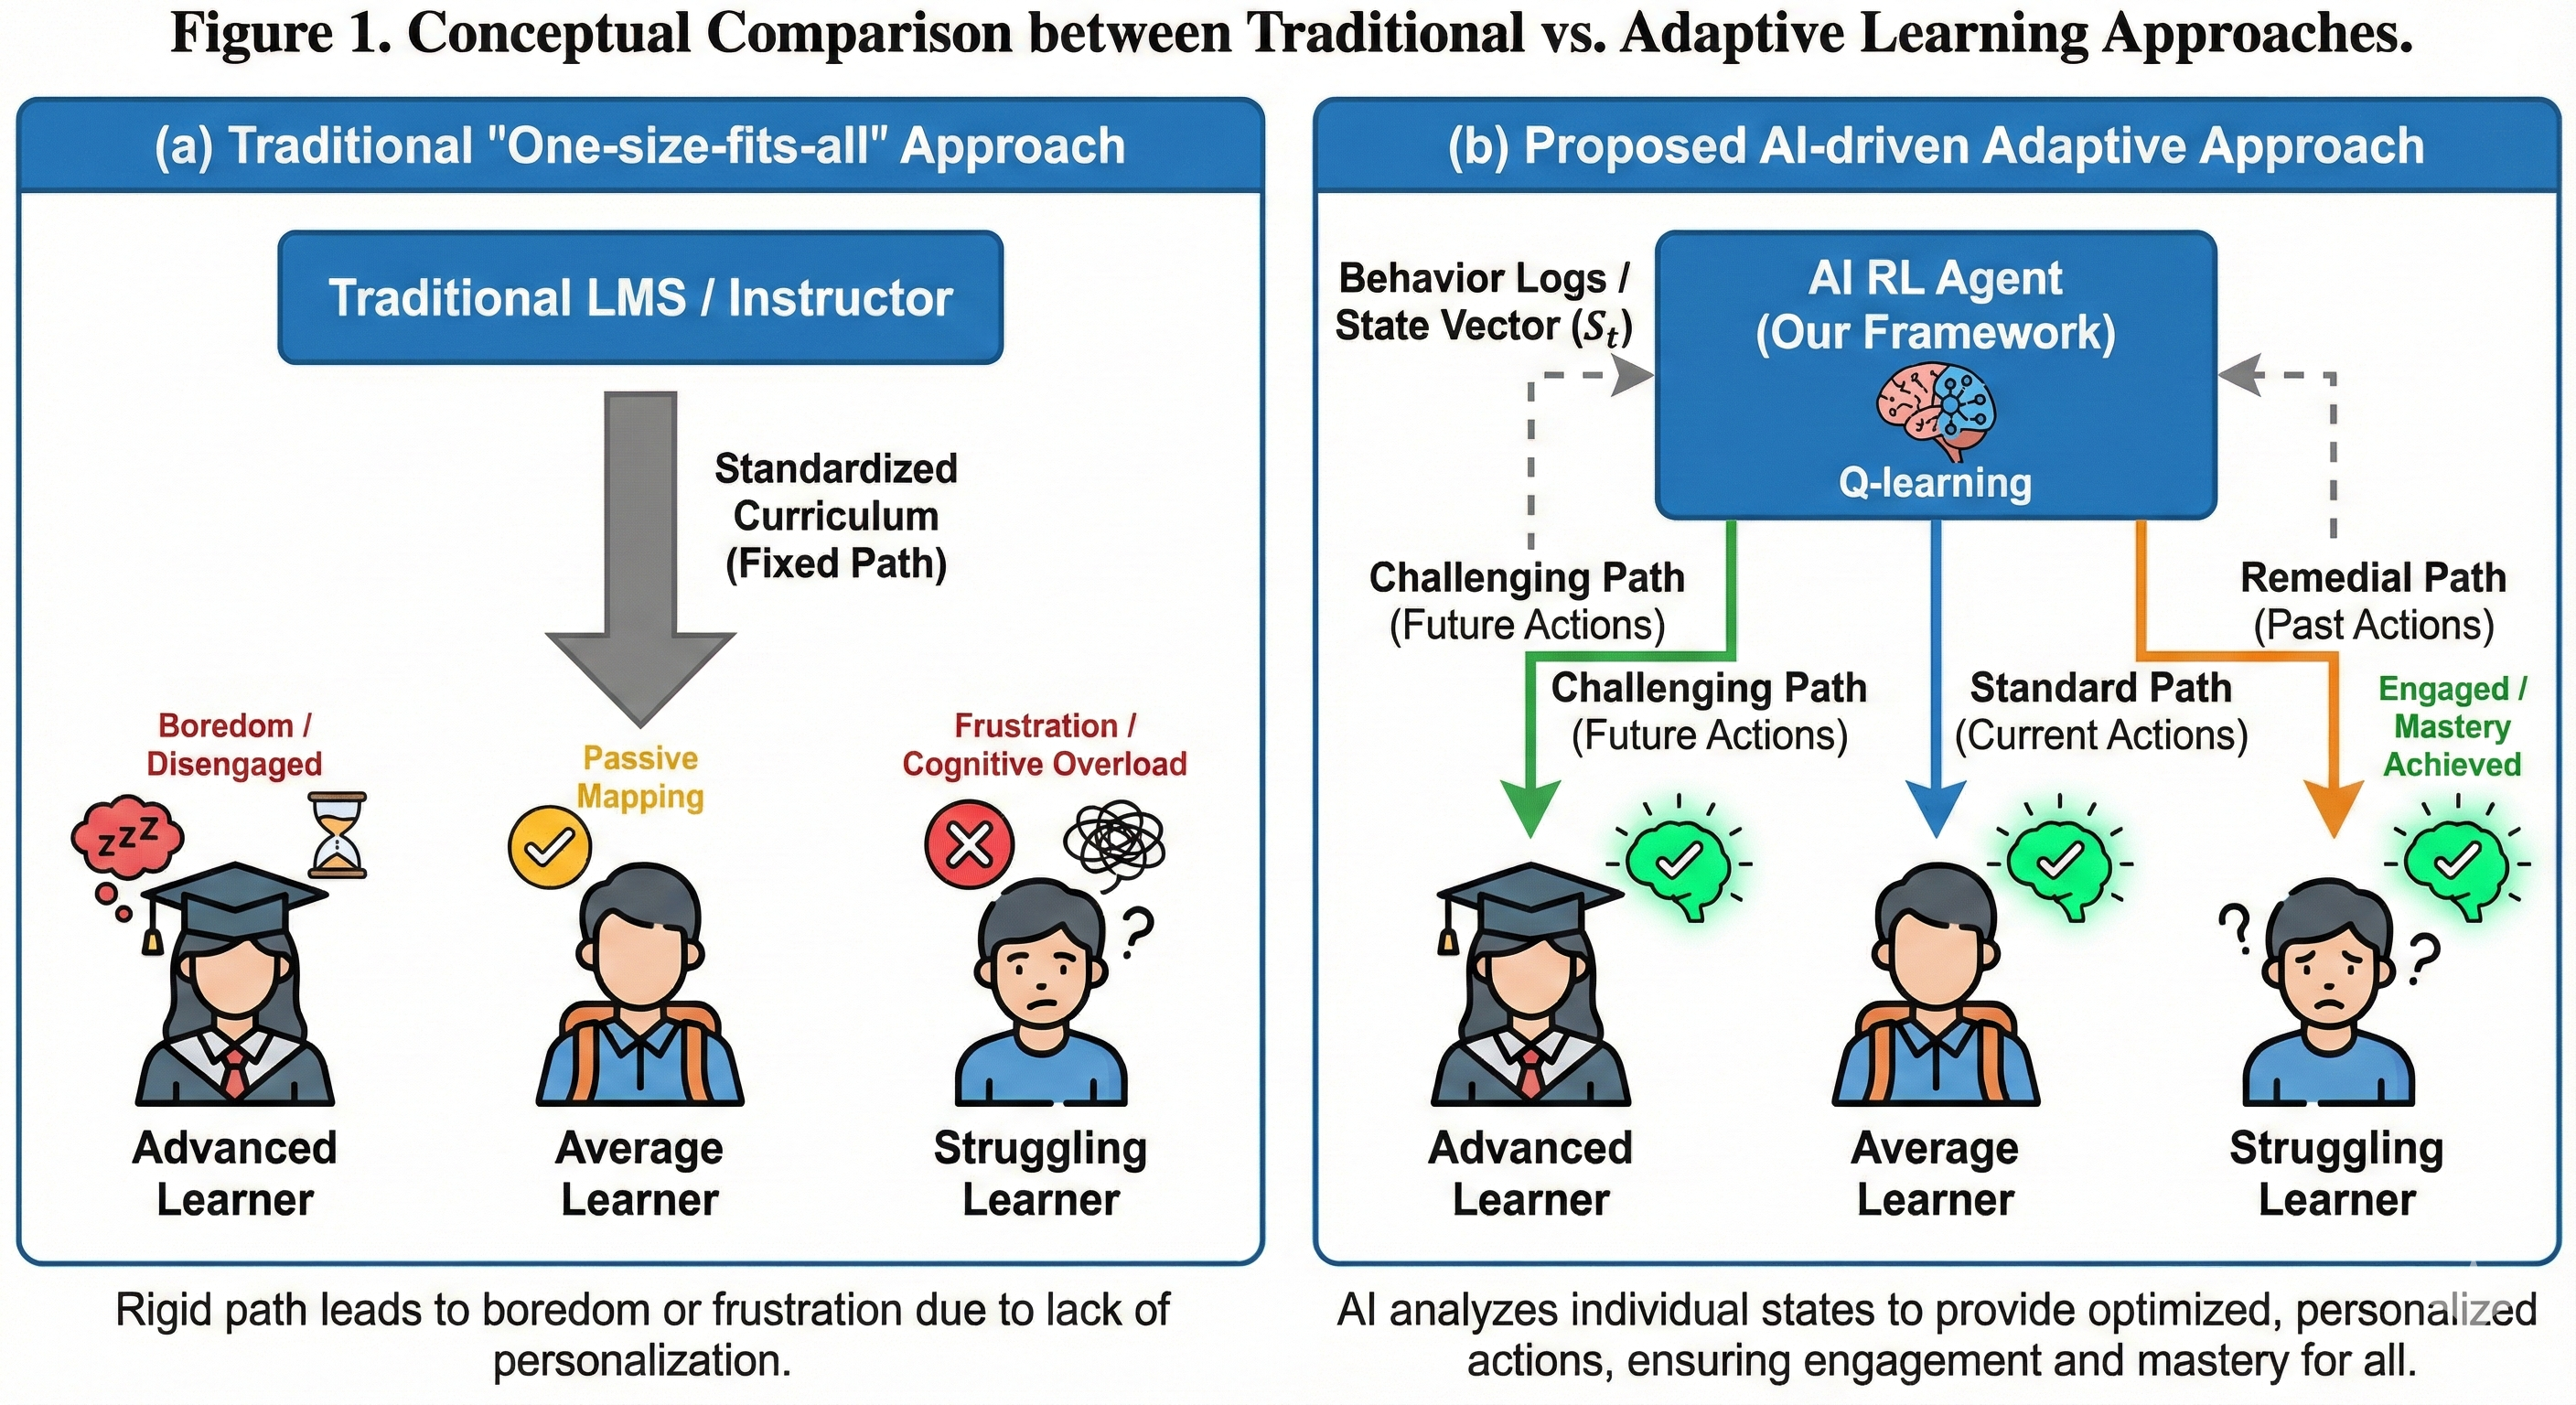
\includegraphics[width=\linewidth]{fig1_problem_concept.pdf}}
\caption{So sánh các phương pháp tiếp cận học tập. (a) Phương pháp truyền thống áp dụng một chương trình cố định cho mọi đối tượng người học, dẫn đến mức độ tương tác không tối ưu (gây nhàm chán hoặc quá tải). (b) Khung giải pháp đề xuất sử dụng Tác nhân Học tăng cường (AI Agent) để phân tích trạng thái người học từ dữ liệu log, từ đó đưa ra các gợi ý hành động cá nhân hóa (ôn tập, tiêu chuẩn, hoặc nâng cao), nhằm tối đa hóa sự tương tác và mức độ thành thạo kiến thức.}
\label{fig:concept}
\end{figure}

\section{Phương pháp Đề xuất}
\label{sec:methodology}

Dựa trên các hạn chế của LMS truyền thống, nghiên cứu đề xuất một khung giải pháp học tập thích ứng (Adaptive Learning Framework) sử dụng thuật toán Q-learning. Quy trình xử lý tổng thể đi từ dữ liệu hành vi thô, qua bước trích xuất đặc trưng để xây dựng không gian trạng thái, và cuối cùng là tác nhân AI đưa ra quyết định tối ưu (Hình \ref{fig:proposed_method}).

% Hình 2: Tổng quan phương pháp (Overview)
\begin{figure}[htbp]
\centerline{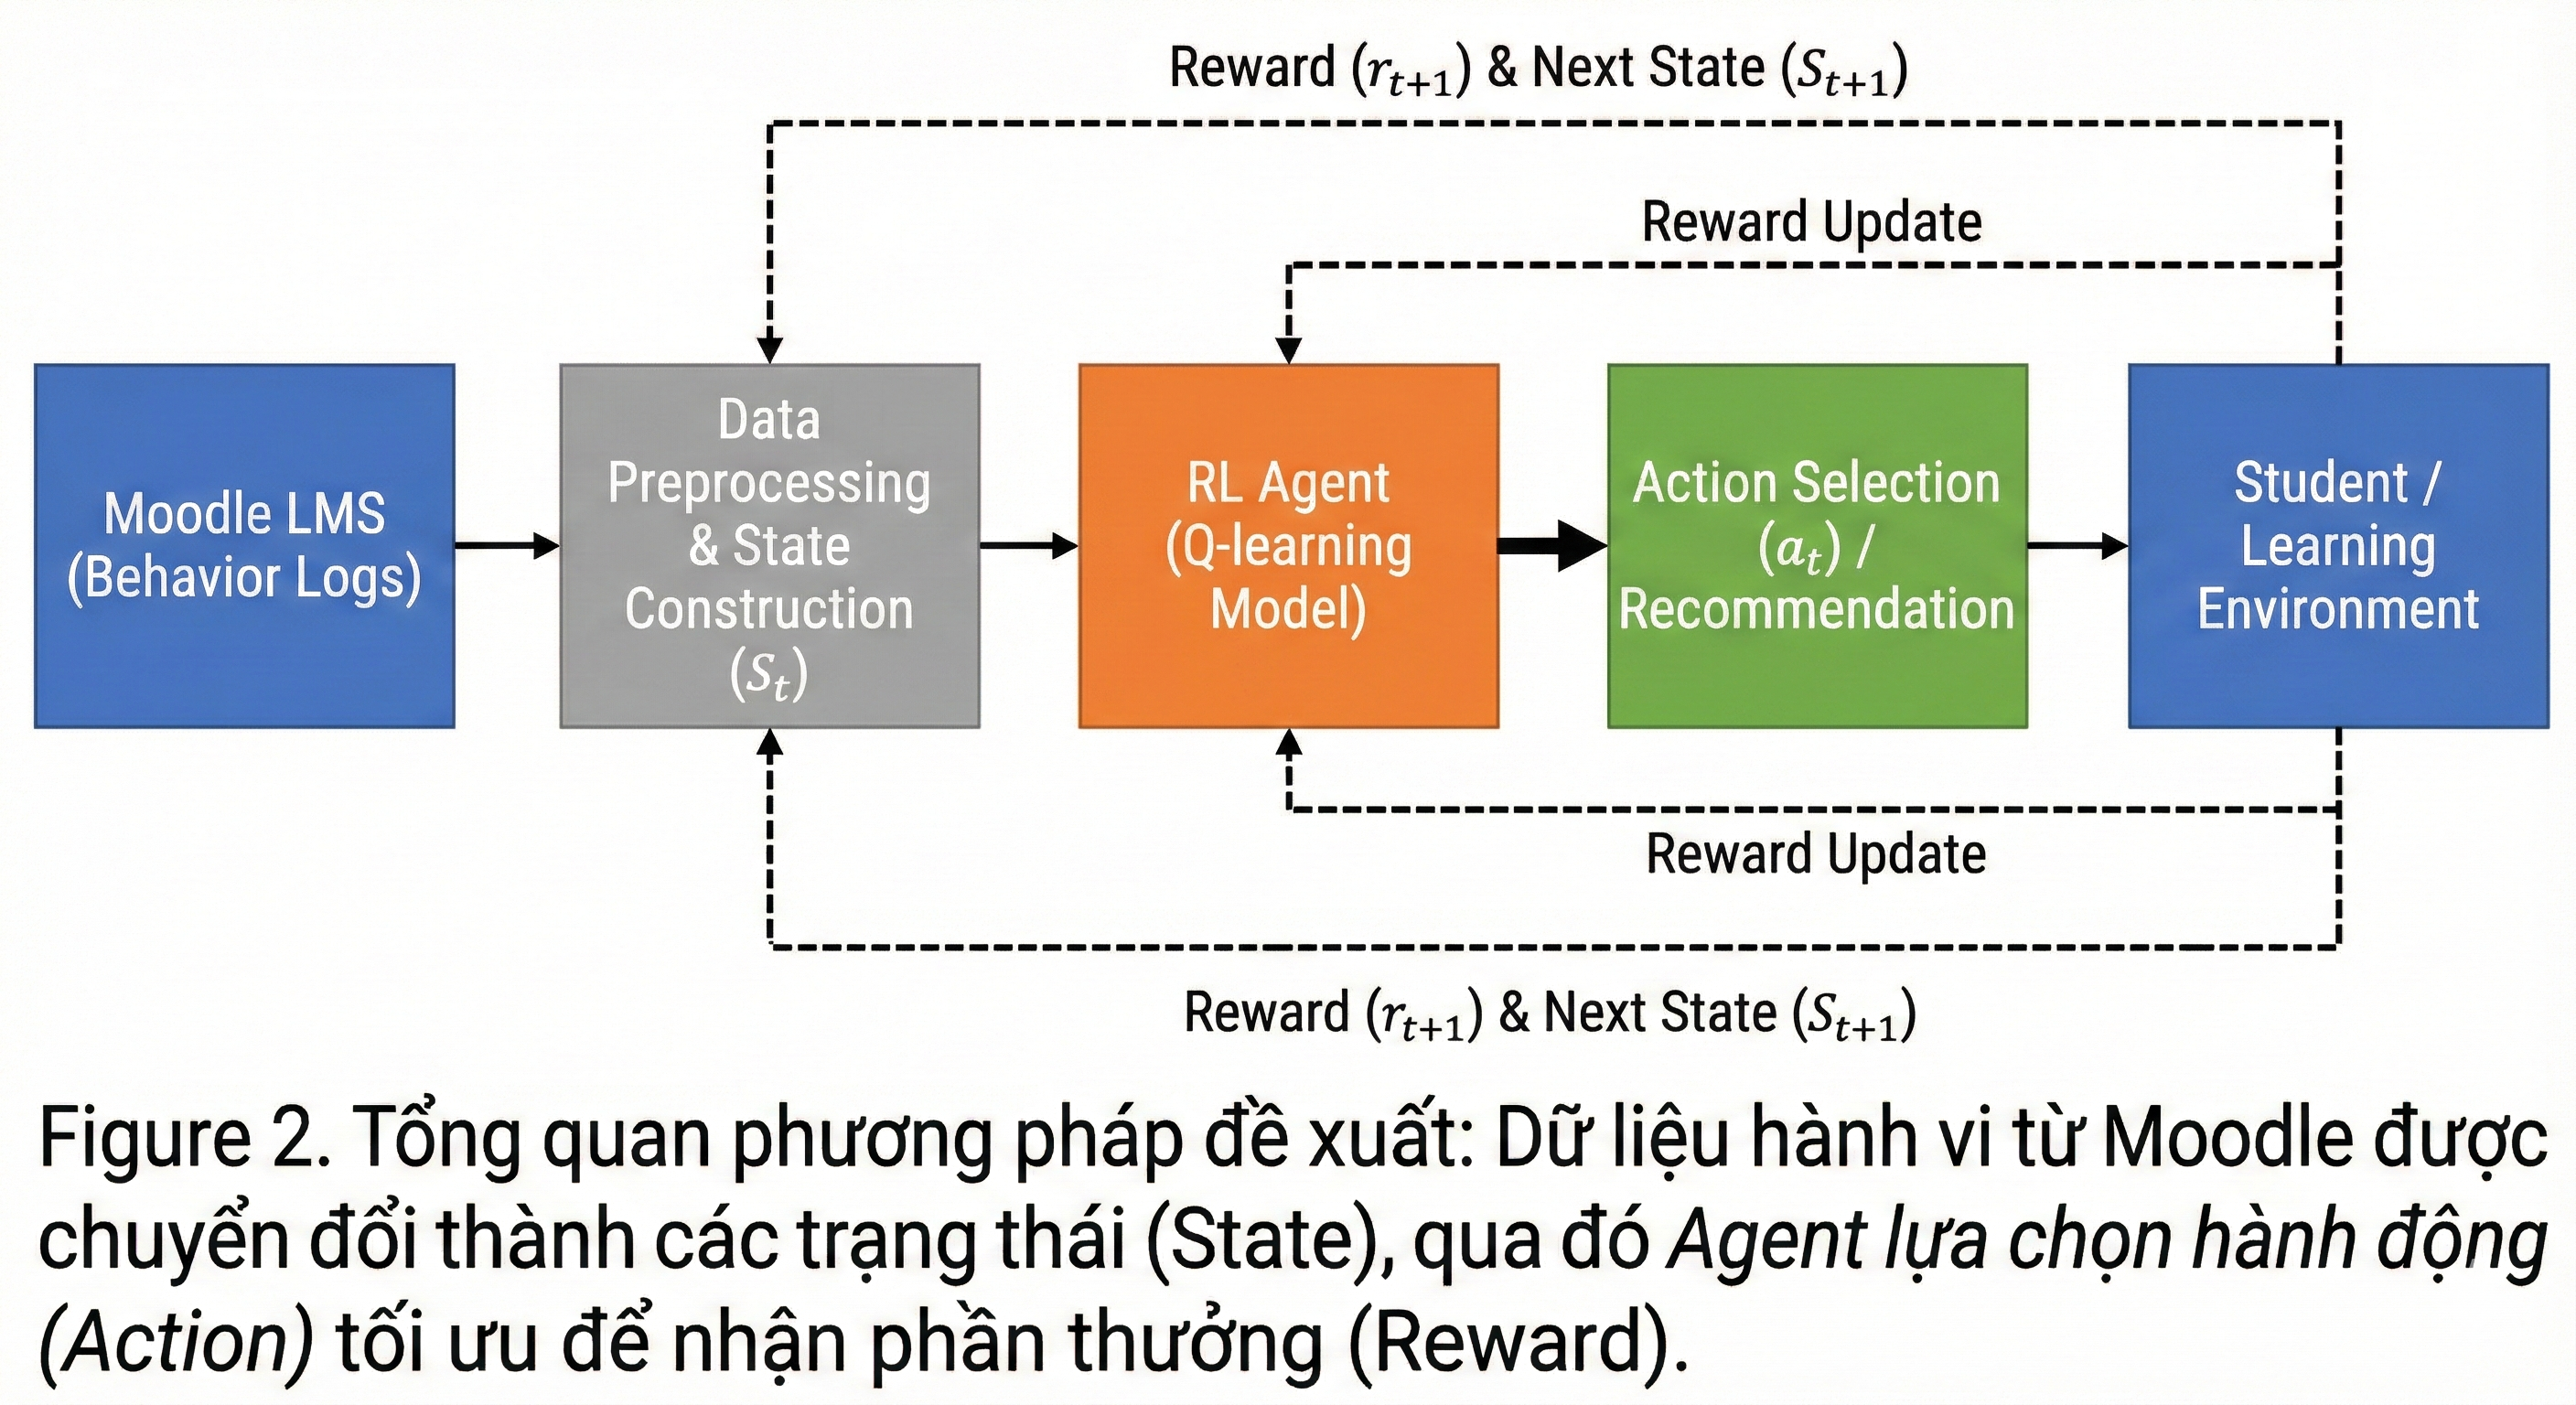
\includegraphics[width=\linewidth]{fig2_method_overview.pdf}}
\caption{Tổng quan phương pháp đề xuất: Dữ liệu hành vi từ Moodle được chuyển đổi thành các trạng thái (State), qua đó Agent lựa chọn hành động (Action) tối ưu để nhận phần thưởng (Reward).}
\label{fig:proposed_method}
\end{figure}

\subsection{Mô hình hóa bài toán (Problem Formulation)}
Để cá nhân hóa lộ trình học tập, chúng tôi mô hình hóa bài toán dưới dạng Quy trình Quyết định Markov (MDP), được định nghĩa bởi bộ ba $<S, A, R>$ như sau:

\subsubsection{Không gian Trạng thái (State Space - $S$)}
Tại thời điểm $t$, hệ thống quan sát trạng thái người học $S_t$. Để đảm bảo tính tổng quát, $S_t$ được định nghĩa là một vector đặc trưng $d$ chiều:
\begin{equation}
S_t = \{f_1, f_2, ..., f_d\}
\end{equation}
Trong nghiên cứu này, chúng tôi đề xuất bộ đặc trưng bao gồm: 
\begin{itemize}
    \item $C$ (Cluster): Nhóm người học xác định qua phân cụm.
    \item $M$ (Module): Chỉ số bài học hiện tại.
    \item $P$ (Progress): Mức độ hoàn thành module.
    \item $Sc$ (Score): Phân loại điểm số tích lũy.
    \item $Ph$ (Phase): Giai đoạn học tập (ví dụ: theo khung ICAP).
    \item $E$ (Engagement): Mức độ tương tác.
\end{itemize}

\subsubsection{Không gian Hành động (Action Space - $A$)}
Dựa trên $S_t$, tác nhân (Agent) lựa chọn một hành động $a_t$ từ tập hợp $A$ gồm $m$ hành động sư phạm khả dĩ ($A = \{a_0, a_1, ..., a_{m-1}\}$). Các hành động này được phân loại theo trục thời gian (Quá khứ - Hiện tại - Tương lai) nhằm phục vụ các chiến lược ôn tập (Remedial) hoặc bồi dưỡng (Advanced).

\subsubsection{Hàm phần thưởng (Reward Function - $R$)}
Mục tiêu của hệ thống là tối đa hóa tổng phần thưởng tích lũy. Hàm thưởng được thiết kế đa mục tiêu:
\begin{equation}
R_{total} = R_{base} + R_{LO} + R_{bonus} - P_{penalty}
\end{equation}
Trong đó, $R_{base}$ là phần thưởng cơ bản, $R_{LO}$ dựa trên mức độ đạt chuẩn đầu ra, $R_{bonus}$ cho các chuỗi hành vi tốt, và $P_{penalty}$ là điểm phạt để hạn chế hành vi kém hiệu quả.

\subsection{Quy trình Xử lý dữ liệu và Phân cụm}
Dữ liệu log thô từ LMS thường chứa nhiễu và không cấu trúc. Trước khi đưa vào mô hình RL, dữ liệu cần được tiền xử lý và chuẩn hóa. Thuật toán K-means được áp dụng để phân chia người học thành $K$ cụm (Clusters) có đặc điểm hành vi tương đồng. Việc xác định giá trị $K$ tối ưu được thực hiện thông qua ba chỉ số đánh giá: phương pháp Elbow (Inertia), chỉ số Silhouette (tách biệt cụm), và chỉ số Davies-Bouldin (độ nén cụm). Kết quả từ ba chỉ số này được hợp nhất bằng cơ chế Bỏ phiếu đa số (Majority Voting) để xác định số cụm tối ưu. Giá trị Cluster ID sau đó trở thành một thành phần quan trọng trong vector trạng thái $S_t$.

\subsection{Thuật toán Q-learning}
Hệ thống sử dụng thuật toán Q-learning để cập nhật bảng giá trị Q (Q-table) theo công thức Bellman:
\begin{equation}
Q(s, a) \leftarrow Q(s, a) + \alpha [r + \gamma \max_{a'} Q(s', a') - Q(s, a)]
\end{equation}
Trong đó $\alpha$ là tốc độ học và $\gamma$ là hệ số chiết khấu. Chiến lược $\epsilon$-greedy được áp dụng để cân bằng giữa khám phá (Exploration) và khai thác (Exploitation).

\begin{figure}[htbp]
\centerline{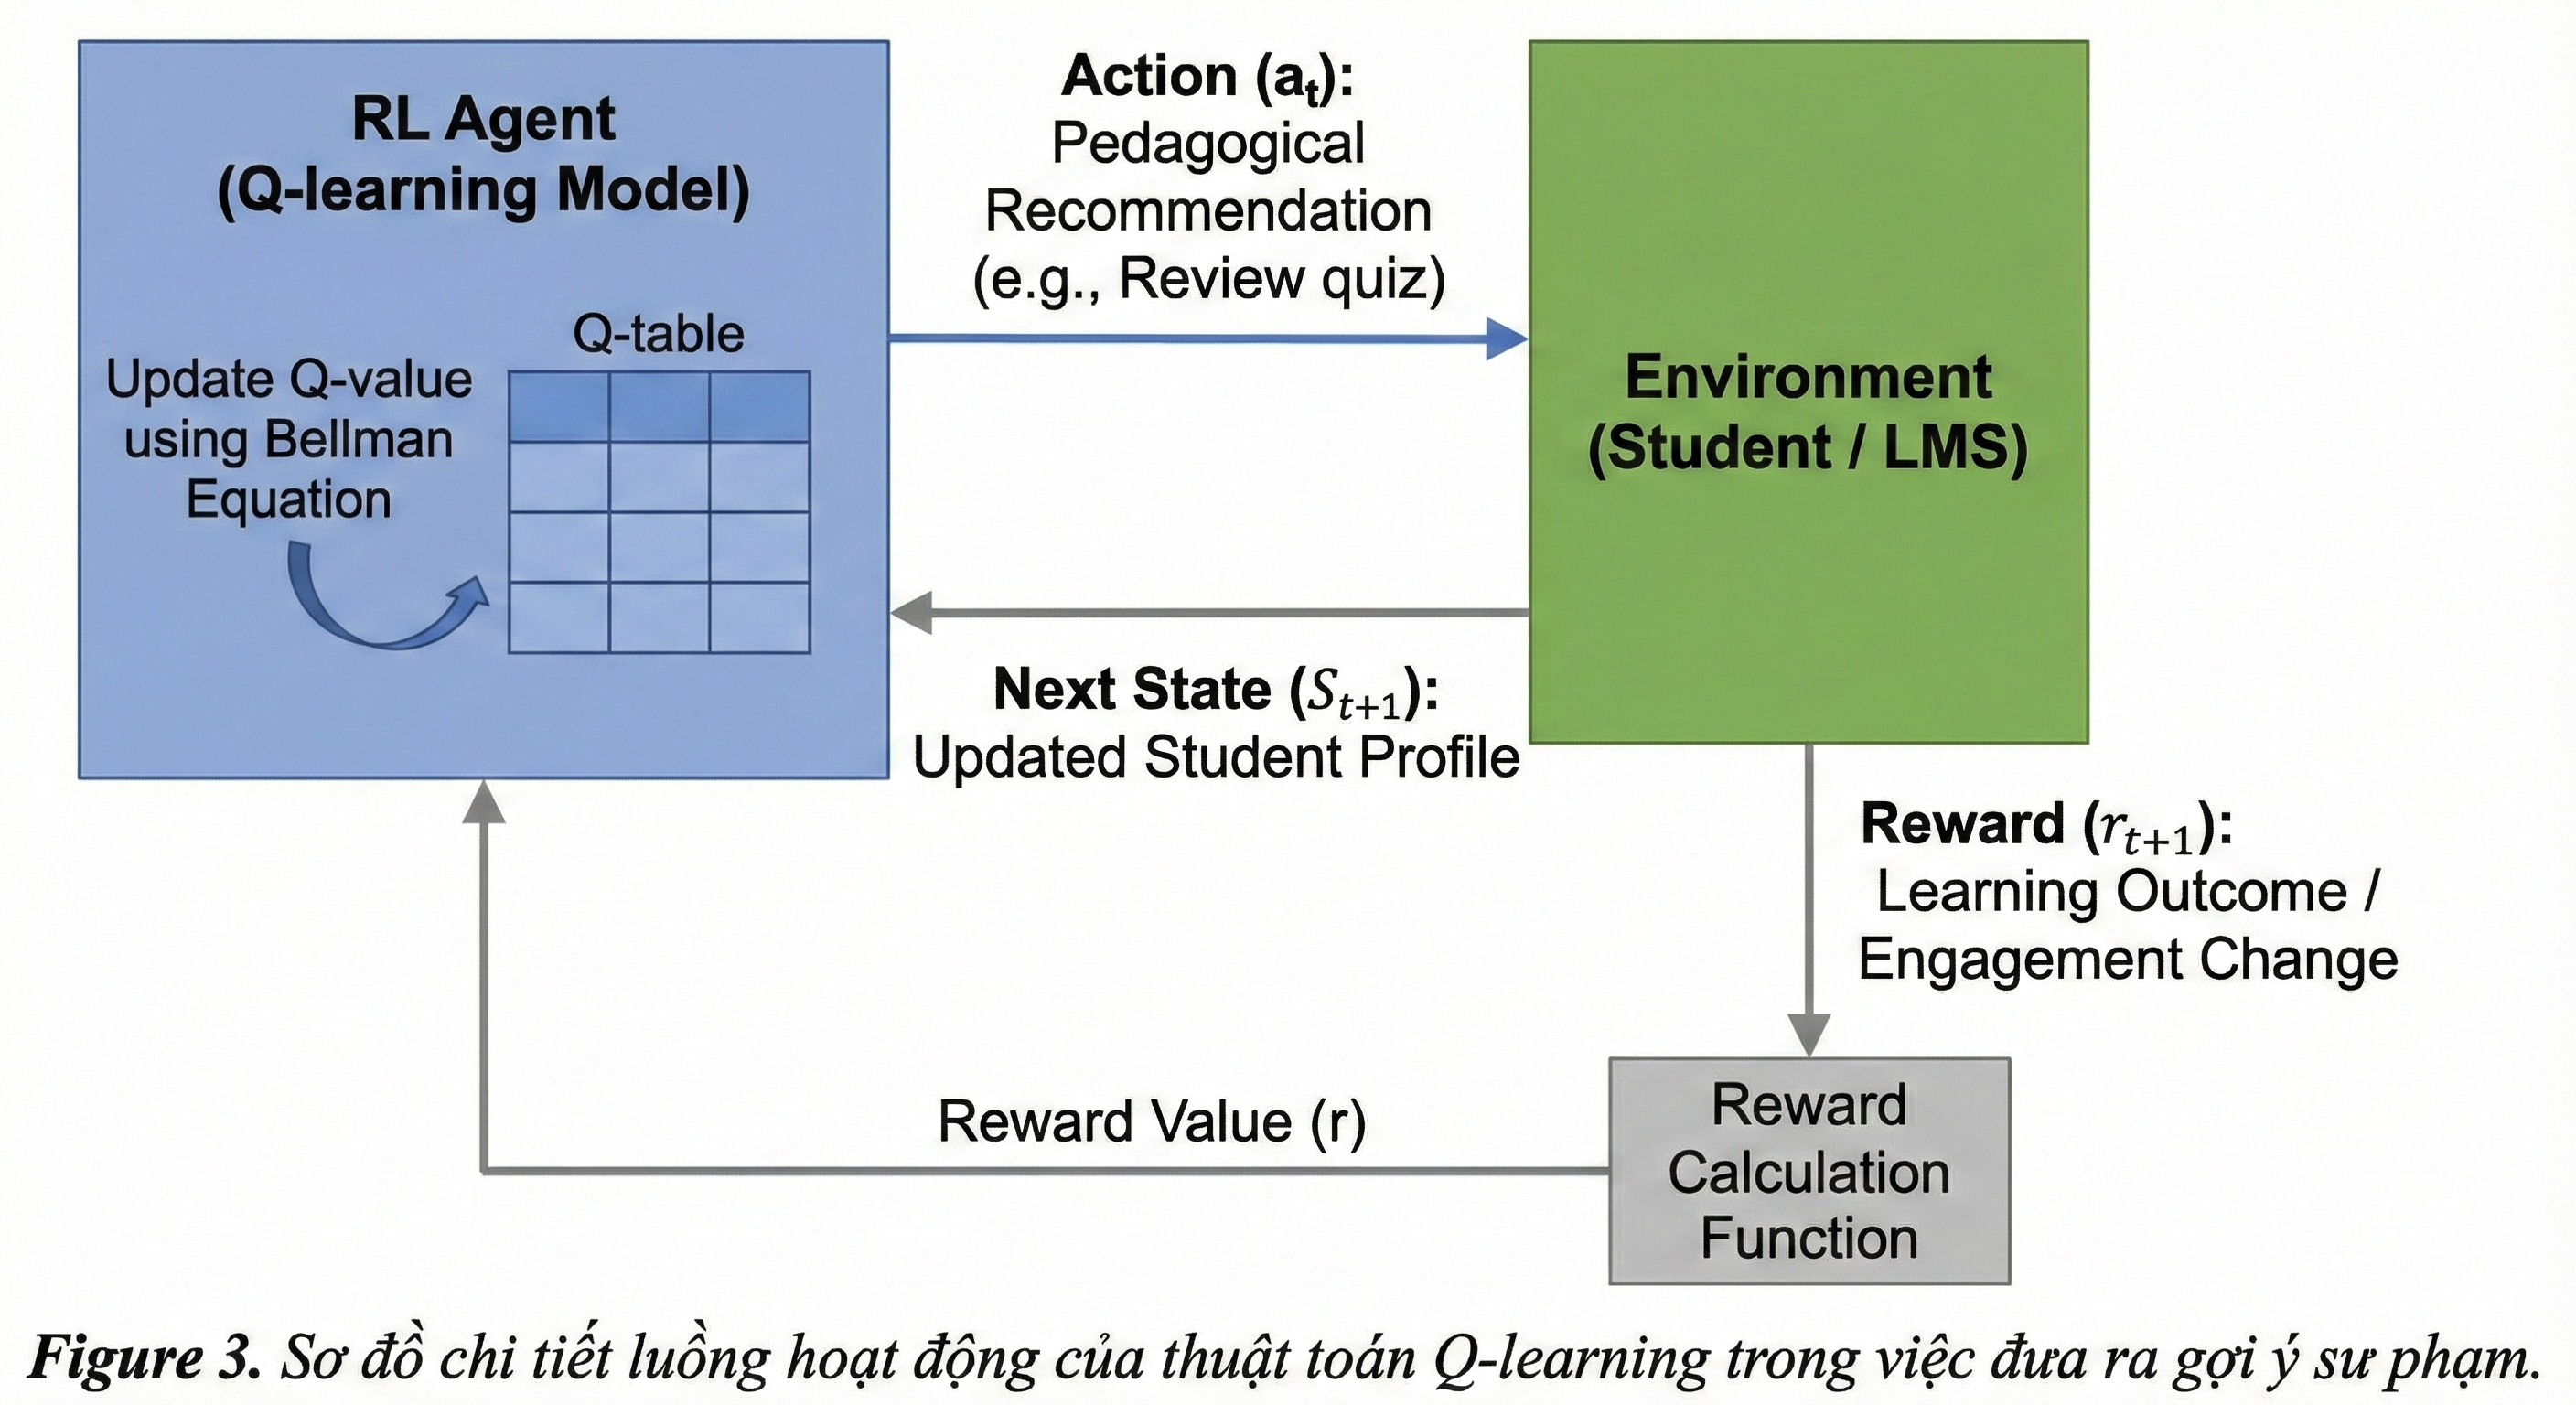
\includegraphics[width=0.9\linewidth]{fig3_qlearning_diagram.pdf}} 
\caption{Sơ đồ chi tiết luồng hoạt động của thuật toán Q-learning trong việc đưa ra gợi ý sư phạm.}
\label{fig:qlearning_diagram}
\end{figure}

\subsection{Khung giải thích mô hình (Explainability Framework)}
Để giải quyết tính ``hộp đen'' của bảng Q-table, nghiên cứu tích hợp phương pháp \textbf{SHAP (SHapley Additive exPlanations)}~\cite{shap_arxiv}.

\subsubsection{Cơ sở toán học}
Giá trị SHAP $\phi_i(s)$ đo lường đóng góp biên của đặc trưng $i$ vào giá trị Q dự đoán:
\begin{equation}
\phi_i(s) = \sum_{S \subseteq F \setminus \{i\}} \frac{|S|!(|F|-|S|-1)!}{|F|!} [f(S \cup \{i\}) - f(S)]
\end{equation}
Tính chất cộng tính đảm bảo: $f(s) = \phi_0 + \sum_{i=1}^{6} \phi_i(s)$. Để đánh giá độ quan trọng toàn cục, chúng tôi tính trung bình trị tuyệt đối SHAP trên một tập mẫu kiểm tra gồm $N$ trạng thái ngẫu nhiên:
\begin{equation}
I_i = \frac{1}{N}\sum_{j=1}^{N}|\phi_i(s_j)|
\end{equation}

\subsubsection{Triển khai kỹ thuật với KernelExplainer}
Quy trình xấp xỉ giá trị Shapley được thực hiện qua 3 bước:
\begin{enumerate}
    \item \textbf{Hàm dự đoán:} Xây dựng hàm wrapper $f(s) = \max_{a} Q(s,a)$, ánh xạ trạng thái $s$ sang giá trị lợi ích tối đa kỳ vọng.
    \item \textbf{Lấy mẫu nền (Background Sampling):} Sử dụng tập dữ liệu nền $D_{bg}$ ($N_{bg}=100$) để đại diện cho kỳ vọng cơ sở $E[f(x)]$.
    \item \textbf{Tính toán (Computation):} Với mỗi trạng thái trong tập kiểm tra, KernelExplainer thực hiện tính toán trên toàn bộ $2^6=64$ liên minh đặc trưng, đảm bảo độ chính xác cao trong thời gian $O(N \cdot 2^D)$.
\end{enumerate}

\subsection{Khung mô phỏng hướng dữ liệu (Data-driven Simulation Framework)}
Để giải quyết bài toán ``khởi động lạnh'' (Cold-start) và đảm bảo tính hội tụ trước khi triển khai thực tế, nghiên cứu đề xuất quy trình \textbf{Khai phá tham số (Parameter Mining)}. Quy trình này chuyển đổi dữ liệu log thô thành các tham số xác suất để vận hành ``Bản sao số'' (Digital Twin) của lớp học thực tế.

\subsubsection{Chiến lược Ánh xạ và Ngữ cảnh hóa}
Hệ thống chuẩn hóa các sự kiện kỹ thuật của Moodle về không gian hành động $A$ gồm 17 hành động chuẩn. Để tăng độ mịn cho không gian trạng thái, mỗi hành động được gắn nhãn ngữ cảnh thời gian dựa trên tiến độ học tập $P_t$:
\begin{equation}
Context(a_t) = \begin{cases} 
\text{Past}, & \text{if } P_t < 25\% \\
\text{Current}, & \text{if } 25\% \le P_t < 85\% \\
\text{Future}, & \text{if } P_t \ge 85\%
\end{cases}
\end{equation}

\subsubsection{Mô hình hóa Xác suất chuyển đổi (Transition Dynamics)}
Dựa trên dữ liệu lịch sử $\mathcal{D}_{history}$, hệ thống xây dựng Ma trận xác suất chuyển đổi (TPM) $\mathcal{P}$. Với mỗi cặp trạng thái - hành động $(s, a)$, xác suất người học chuyển sang trạng thái tiếp theo $s'$ được ước lượng bởi:
\begin{equation}
P(s' | s, a) = \frac{count(s, a, s')}{\sum_{s^*} count(s, a, s^*)}
\end{equation}
Ma trận $\mathcal{P}$ đóng vai trò là quy luật vận hành của môi trường, đảm bảo phản ứng của hệ thống giả lập sát với thực tế.

\subsubsection{Mô hình hóa Chính sách Đối chứng (Param Policy Baseline)}
Để đánh giá hiệu quả, chúng tôi xây dựng một \textbf{Param Policy} ($\pi_{param}$) làm baseline so sánh. Đây là chính sách tham số hóa (parametric policy) dựa trên phân phối xác suất hành động từ dữ liệu lịch sử, mô phỏng lại thói quen tự nhiên của sinh viên trong quá khứ:
\begin{equation}
\begin{aligned}
\pi_{param}(a|s) &= P(a \mid \text{Phase}(s), \text{Cluster}(s)) \\
&= \frac{\text{count}\big(\text{Phase}(s), \text{Cluster}(s), a\big)}
        {\sum_{a'} \text{count}\big(\text{Phase}(s), \text{Cluster}(s), a'\big)}
\end{aligned}
\end{equation}
Với mỗi trạng thái $s$, hành động được gợi ý dựa trên tần suất xuất hiện trong tập huấn luyện, phân tầng theo giai đoạn học tập (Phase) và nhóm người học (Cluster). Đây là baseline để so sánh với chiến lược tối ưu hóa phần thưởng ($\pi^*$) của Q-learning.

\subsubsection{Quy trình Huấn luyện và Đánh giá}
Quy trình mô phỏng được thực hiện theo chu trình khép kín:
\begin{enumerate}
    \item \textbf{Khởi tạo (Initialization):} Thiết lập các Tác nhân Người học (Student Agents) với đặc trưng hành vi được tham số hóa từ các cụm dữ liệu (Clusters).
    \item \textbf{Huấn luyện (Training):} Agent tương tác với Student Agents trong môi trường $\mathcal{P}$ để tối ưu bảng Q-table thông qua cơ chế thử-sai.
    \item \textbf{Đối sánh (Comparison):} So sánh hiệu suất (Reward, Score, LO Mastery) giữa chiến lược tối ưu $\pi^*$ của Q-learning Agent và chính sách đối chứng $\pi_{param}$ (Param Policy baseline).
\end{enumerate}

\section{Thực nghiệm và Kết quả}
\label{sec:experiments}

\subsection{Thiết lập Môi trường Giả lập (Simulation Setup)}

\subsubsection{Mô hình hóa Phong cách học tập}
Các tác nhân ảo (Virtual Agents) không hành động ngẫu nhiên mà sở hữu các phong cách học tập phi tuyến tính. Phân phối phong cách được thiết lập dựa trên tham số thực tế:
\begin{itemize}
    \item \textbf{Linear Learner (70\%):} Tuân thủ lộ trình tuần tự truyền thống.
    \item \textbf{Practice-first (10\%):} Ưu tiên thực hiện bài tập/quiz trước khi xem lý thuyết.
    \item \textbf{Video/Reading-first (20\%):} Ưu tiên tiêu thụ nội dung thụ động trước khi tương tác.
\end{itemize}

\subsubsection{Cấu hình Ngẫu nhiên và Tham số Mô phỏng (Simulation Settings \& Stochasticity)}
Để đảm bảo tính khách quan và khả năng tái lập (reproducibility) của thực nghiệm, môi trường mô phỏng được thiết lập với các tham số chi tiết về nhiễu (noise) và quy mô mẫu như sau:

\textbf{1) Quy mô và Tái lập:}
Quá trình huấn luyện diễn ra qua 500 episodes. Trong mỗi episode, hệ thống khởi tạo một quần thể gồm 100 tác nhân người học ảo (Student Agents). Như vậy, Agent được học từ tổng cộng $50,000$ lượt tương tác mô phỏng, đảm bảo độ bao phủ không gian trạng thái. 
Hạt giống ngẫu nhiên (Random Seed) được cố định ở giá trị $42$ để đảm bảo sự nhất quán giữa các lần chạy thử nghiệm.

\textbf{2) Mô hình Nhiễu (Noise Modeling):}
Mô phỏng tích hợp tính ngẫu nhiên để phản ánh sự biến thiên trong hành vi thực tế của sinh viên.
\begin{itemize}
    \item \textbf{Biến thiên Điểm số ($\sigma$):} Điểm số đạt được sau mỗi hành động không cố định mà chịu tác động của nhiễu phân phối đều (Uniform Noise). Công thức tính điểm thực tế $S_{real}$ được định nghĩa:
    \begin{equation}
        S_{real} = \text{clip}(S_{base} + \mathcal{U}(-\sigma_c, \sigma_c), 0, 1)
    \end{equation}
    Trong đó $\sigma_c$ là độ biến thiên đặc trưng cho từng cụm: Nhóm Yếu có độ biến động cao nhất ($\sigma=0.18$), tiếp theo là Trung bình ($\sigma=0.10$) và Thấp nhất ở nhóm Giỏi ($\sigma=0.05$).
    
    \item \textbf{Biến thiên Thời gian:} Thời gian hoàn thành một hành động được lấy mẫu ngẫu nhiên trong khoảng từ 5 đến 30 phút để mô phỏng sự chênh lệch về tốc độ xử lý thông tin: $T \sim \mathcal{U}(5, 30)$[cite: 1441].
\end{itemize}

\textbf{3) Điều kiện dừng (Termination):}
Mỗi episode kết thúc khi tác nhân người học hoàn thành toàn bộ $N=6$ module của khóa học hoặc khi đạt giới hạn bước tối đa (max steps = 100) để ngăn chặn các vòng lặp vô tận trong giai đoạn đầu của quá trình thăm dò (exploration)[cite: 1183, 1516].

\begin{table}[htbp]
\caption{Tổng hợp tham số cấu hình mô phỏng}\label{tab:sim_params}
\begin{center}
\begin{tabular}{lp{4.5cm}c}
\toprule
\textbf{Tham số} & \textbf{Mô tả} & \textbf{Giá trị} \\
\midrule
$N_{episodes}$ & Số lượng vòng lặp huấn luyện & 500 \\
$Seed$ & Hạt giống ngẫu nhiên & 42 \\
$N_{modules}$ & Số module trong khóa học & 6 \\
\midrule
\multicolumn{3}{l}{\textit{Tham số theo phân cụm:}} \\
$P_{success}$ (Weak) & Xác suất thành công cơ sở & 0.72 \\
$P_{success}$ (Medium) & Xác suất thành công cơ sở & 0.78 \\
$P_{success}$ (Strong) & Xác suất thành công cơ sở & 0.90 \\
$\alpha_{learn}$ (Weak) & Tốc độ học tập & 0.22 \\
$\alpha_{learn}$ (Medium) & Tốc độ học tập & 0.32 \\
$\alpha_{learn}$ (Strong) & Tốc độ học tập & 0.30 \\
\bottomrule
\end{tabular}
\end{center}
\end{table}

\subsection{Thiết lập thực nghiệm (Experimental Setup)}

\subsubsection{Dữ liệu huấn luyện (Dataset Ground Truth)}
Nghiên cứu sử dụng bộ dữ liệu chuẩn \textit{Moodle Log \& Grades} \cite{dataset_kaggle}. Trong số các khóa học có sẵn, chúng tôi lựa chọn \textbf{Khóa học ID 670} làm cơ sở để xây dựng môi trường mô phỏng (Data-driven Environment).

Quyết định này dựa trên sự cân bằng lý tưởng của dữ liệu: Khóa học ghi nhận 13,995 điểm tương tác từ 23 sinh viên với phân phối điểm số chuẩn ($\mu=7.64, \sigma=2.95$). Điều này khắc phục được hạn chế dữ liệu bị lệch (skewed data) thường thấy ở các khóa học khác (ví dụ Course ID 42 có Mean=1.07), giúp thuật toán phân biệt rõ ràng chiến lược học tập giữa các nhóm sinh viên (Giỏi, Khá, Yếu).

\subsubsection{Quy trình Tiền xử lý và Phân cụm (Data Preprocessing \& Clustering)}
Hệ thống sử dụng thuật toán K-Means nhờ ưu thế về tốc độ xử lý dữ liệu số. Để đảm bảo tính chính xác và tránh chọn tham số chủ quan, nghiên cứu áp dụng quy trình lọc hai lớp kết hợp với cơ chế ``Bỏ phiếu đa số'' (Majority Voting) để xác định cấu trúc phân nhóm.

\textbf{1) Chọn lọc đặc trưng (Feature Selection):}
Dữ liệu đầu vào được chuẩn hóa (Z-score normalization), sau đó đi qua bộ lọc hai lớp để tinh gọn không gian chiều:
\begin{itemize}
    \item \textbf{Lọc phương sai (Variance Filtering):} Loại bỏ các đặc trưng có phương sai dưới ngưỡng $0.01$ (ít biến động, không mang giá trị phân loại).
    \item \textbf{Lọc tương quan (Correlation Filtering):} Với ngưỡng tương quan Pearson $> 0.95$, thuật toán đã loại bỏ \textbf{78 đặc trưng} bị trùng lặp thông tin, giải quyết triệt để hiện tượng đa cộng tuyến.
\end{itemize}

\textbf{2) Tối ưu hóa số cụm ($K$):}
Số lượng cụm $K$ được quyết định dựa trên sự đồng thuận của 3 chỉ số đánh giá độ gom cụm (Hình \ref{fig:clustering_metrics}):
\begin{itemize}
    \item \textbf{Elbow Method:} Biểu đồ độ lỗi (Inertia) xuất hiện điểm uốn (knee point) rõ nét tại $K=6$.
    \item \textbf{Silhouette Score:} Đạt giá trị cực đại tại $K=2$ ($0.42$). Tuy nhiên, tại $K=6$, chỉ số này vẫn duy trì mức ổn định chấp nhận được ($\approx 0.35$).
    \item \textbf{Davies-Bouldin Index:} Chỉ số đo độ nén (càng thấp càng tốt) cho thấy điểm trũng cục bộ khả quan tại $K=6$.
\end{itemize}

\begin{figure}[htbp]
\centerline{\includegraphics[width=\columnwidth]{fig4_clustering_metrics.pdf}} 
\caption{Các chỉ số đánh giá phân cụm. Elbow và Davies-Bouldin ủng hộ $K=6$, trong khi Silhouette chấp nhận được ở ngưỡng này.}
\label{fig:clustering_metrics}
\end{figure}

\textbf{3) Biện luận lựa chọn $K=6$:}
Mặc dù $K=2$ cho chỉ số tách biệt tốt nhất, nhưng việc phân chia sinh viên chỉ thành 2 nhóm (Giỏi/Yếu) là quá thô sơ, không đủ độ mịn để Agent tối ưu hóa chiến lược sư phạm. Ngược lại, $K \ge 10$ quá phức tạp và gây bùng nổ không gian trạng thái (State Explosion). Do đó, $K=6$ là điểm cân bằng tối ưu, đại diện cho 6 hồ sơ năng lực điển hình của người học.

Trong quá trình phân tích cụm, một cụm được phát hiện là đại diện cho hành vi của giảng viên (tần suất cao các sự kiện chấm điểm và hoạt động diễn đàn). Cụm này được loại bỏ khỏi tập dữ liệu huấn luyện của Agent, chỉ giữ lại 5 cụm hành vi sinh viên. Các cụm sinh viên này sau đó được ánh xạ về ba nhóm sư phạm (Weak, Medium, Strong) để cấu hình hàm phần thưởng thích ứng.

\subsubsection{Mô hình hóa Quy luật Chuyển đổi và Chính sách Đối chứng (Transition Dynamics \& Baseline)}
Tính hợp lý của môi trường mô phỏng (Bản sao số) được xác định bởi Ma trận xác suất chuyển trạng thái. Kết quả khai phá dữ liệu (Parameter Mining) từ tập huấn luyện được định lượng chi tiết thông qua các bảng phân phối xác suất, đóng vai trò là tham số đầu vào cho chính sách đối chứng Param Policy ($\pi_{param}$).

\textbf{1) Phân phối hành động theo Giai đoạn học tập (Learning Phase):}
Dữ liệu tại Bảng \ref{tab:phase_probs} cho thấy sự chuyển dịch hành vi rõ rệt giữa các giai đoạn, từ thụ động sang kiến tạo và cuối cùng là phản tư.

\begin{table}[htbp]
\caption{Xác suất chọn hành động theo Giai đoạn (Learning Phase)}\label{tab:phase_probs}
\begin{center}
\begin{tabular}{llc}
\toprule
\textbf{Giai đoạn} & \textbf{Hành động ($a_t$)} & \textbf{Xác suất ($P$)} \\
\midrule
\multirow{2}{*}{Phase 0 (Pre-learning)} & view\_assignment & 56.4\% \\
 & view\_content & 43.6\% \\
\midrule
\multirow{2}{*}{Phase 1 (Active)} & \textbf{attempt\_quiz} & \textbf{74.4\%} \\
 & submit\_assignment & 25.6\% \\
\midrule
Phase 2 (Reflective) & post\_forum & 100.0\% \\
\bottomrule
\end{tabular}
\end{center}
\end{table}

\textbf{2) Phân phối theo Mức độ Tương tác (Engagement Level):}
Bảng \ref{tab:engage_probs} thể hiện sự phân hóa trong chiến lược chọn hành động giữa các nhóm sinh viên. Nhóm tương tác cao (High) có xu hướng duy trì cân bằng giữa xem nội dung và làm bài tập, trong khi nhóm thấp (Low) tập trung chủ yếu vào việc xem yêu cầu bài tập (\textit{view\_assignment}).

\begin{table}[htbp]
\caption{Phân phối xác suất hành động theo Mức độ tương tác}\label{tab:engage_probs}
\begin{center}
\resizebox{\columnwidth}{!}{% Resize bảng để vừa khít cột báo
\begin{tabular}{lccccc}
\toprule
\textbf{Mức độ} & \textbf{View Assign} & \textbf{View Content} & \textbf{Quiz} & \textbf{Submit} & \textbf{Forum} \\
\midrule
\textbf{High} & 52.2\% & 40.5\% & 5.8\% & 1.5\% & 0.02\% \\
\textbf{Medium} & 51.7\% & 41.9\% & 4.3\% & 2.2\% & - \\
\textbf{Low} & \textbf{57.6\%} & 34.0\% & 4.8\% & 3.6\% & - \\
\bottomrule
\end{tabular}
}
\end{center}
\end{table}

Các tham số này được xuất ra dưới dạng cấu hình JSON để điều khiển hành vi ngẫu nhiên có hướng của các Tác nhân người học (Student Agents) trong quá trình mô phỏng.

\subsubsection{Tham số mô hình (Model Parameters)}
Trong quá trình thực nghiệm, các tham số mô hình được thiết lập chi tiết để đảm bảo sự hội tụ của thuật toán:

\begin{itemize}
    \item \textbf{Không gian trạng thái ($S$):} Trạng thái $S_t$ được định nghĩa là vector 6 chiều phản ánh ngữ cảnh người học:
    \begin{equation}
    S_t = (C, M, P, Sc, Ph, E)
    \end{equation}
    Trong đó: $C$ là chỉ số cụm hành vi sinh viên được suy ra từ mô hình K-means ban đầu với $K=6$; sau khi loại bỏ một cụm ứng với hành vi giảng viên, còn lại 5 cụm sinh viên ($C \in \{0,1,2,3,4\}$) được mã hóa vào không gian trạng thái. $M$ là chỉ số module; $P, Sc$ là mức tiến độ và điểm số (rời rạc hóa 4 mức); $Ph$ là giai đoạn học tập ($0$: Pre, $1$: Active, $2$: Reflective); và $E$ là mức độ tương tác (Low, Med, High). Kích thước không gian là $5 \times 6 \times 4 \times 4 \times 3 \times 3 \approx 4,320$ trạng thái.

    \item \textbf{Không gian hành động ($A$):} Gồm $m=15$ hành động được sàng lọc qua bộ lọc ICAP và Pareto ($>1\%$ tần suất). Để tối ưu hiển thị, các hành động được nhóm theo ngữ cảnh thời gian như trình bày tại Bảng \ref{tab:action_space_compact}.

    \item \textbf{Tham số Q-learning:} Tốc độ học $\alpha=0.1$, hệ số chiết khấu $\gamma=0.95$, và chiến lược $\epsilon$-greedy giảm dần.
\end{itemize}

\subsection{Mô hình hóa Không gian trạng thái (State Space Definition)}
Bài toán được mô hình hóa dưới dạng Quy trình Quyết định Markov (MDP). Trạng thái $S_t$ tại thời điểm $t$ là một vector 6 chiều, kết hợp giữa đặc điểm phân cụm cố định và các biến hành vi động:
\begin{equation}
S_t = (C, M, P, Sc, Ph, E)
\end{equation}

Để đảm bảo khả năng hội tụ của bảng Q-table trong giới hạn tính toán, các biến trạng thái liên tục được rời rạc hóa (discretized) theo các ngưỡng sư phạm cụ thể, được chi tiết hóa tại Bảng \ref{tab:state_space_detail}.

\begin{table}[htbp]
\caption{Định nghĩa chi tiết và Miền giá trị của Không gian trạng thái}\label{tab:state_space_detail}
\begin{center}
\resizebox{\columnwidth}{!}{%
\begin{tabular}{l|l|l|c}
\toprule
\textbf{Ký hiệu} & \textbf{Thành phần} & \textbf{Định nghĩa / Rời rạc hóa (Bins)} & \textbf{Kích thước} \\
\midrule
$C$ & Cluster & Nhóm hành vi sinh viên sau khi loại bỏ cụm giảng viên từ mô hình K-means ban đầu ($ID \in \{0, 1, 2, 3, 4\}$) & 5 \\
\midrule
$M$ & Module & Chỉ số bài học hiện tại ($ID \in \{0, \dots, 5\}$) & 6 \\
\midrule
\multirow{4}{*}{$P$} & \multirow{4}{*}{Progress} & Mức 0.25: Mới bắt đầu ($< 25\%$) & \multirow{4}{*}{4} \\
 & & Mức 0.50: Đang học ($25\% - 50\%$) & \\
 & & Mức 0.75: Gần xong ($50\% - 99\%$) & \\
 & & Mức 1.00: Hoàn thành ($100\%$) & \\
\midrule
\multirow{4}{*}{$Sc$} & \multirow{4}{*}{Score} & Mức 0.25 (Yếu): $< 2.5$ & \multirow{4}{*}{4} \\
 & & Mức 0.50 (TB): $2.5 \le s < 5.0$ & \\
 & & Mức 0.75 (Khá): $5.0 \le s < 7.5$ & \\
 & & Mức 1.00 (Giỏi): $\ge 7.5$ & \\
\midrule
\multirow{3}{*}{$Ph$} & \multirow{3}{*}{Phase} & 0: Pre-learning (Tiếp thu thụ động) & \multirow{3}{*}{3} \\
 & & 1: Active-learning (Tương tác/Làm bài) & \\
 & & 2: Reflective-learning (Ôn tập/Thảo luận) & \\
\midrule
\multirow{3}{*}{$E$} & \multirow{3}{*}{Engagement} & 0: Thấp ($S_{total} < 8$) & \multirow{3}{*}{3} \\
 & & 1: Trung bình ($8 \le S_{total} < 16$) & \\
 & & 2: Cao ($S_{total} \ge 16$) & \\
\bottomrule
\end{tabular}
}
\end{center}
\end{table}

\subsubsection{Cơ chế tính toán mức độ tương tác (Engagement Calculation)}
Khác với các nghiên cứu trước chỉ đếm số lượng hành động, chúng tôi đề xuất công thức tính điểm tương tác tổng hợp $S_{total}$ dựa trên khung lý thuyết ICAP, kết hợp ba yếu tố: trọng số hành động, thời gian và tính nhất quán.

\begin{equation}
S_{total} = S_{weighted} + S_{time} + S_{consistency}
\end{equation}

Trong đó:
\begin{itemize}
    \item \textbf{$S_{weighted}$ (Chất lượng hành động):} Tổng trọng số ICAP của các hành động trong cửa sổ quan sát. Các hành động kiến tạo (như \textit{submit\_assignment}) có trọng số cao ($w=5$), trong khi hành động thụ động (như \textit{view}) có trọng số thấp ($w=1$):
    $$ S_{weighted} = \sum_{i=1}^{n} w(action_i) $$
    
    \item \textbf{$S_{time}$ (Hiệu quả thời gian):} So sánh thời gian thực tế $T_{real}$ với thời gian kỳ vọng $T_{exp}$:
    $$ S_{time} = \begin{cases} 
    2 & \text{if } T_{real} \ge 50\% T_{exp} \\
    1 & \text{if } 30\% \le T_{real} < 50\% T_{exp} \\
    0 & \text{else}
    \end{cases} $$
    
    \item \textbf{$S_{consistency}$ (Tính đều đặn):} Dựa trên khoảng cách trung bình $\Delta t$ giữa các lần tương tác:
    $$ S_{consistency} = \begin{cases} 
    2 & \text{if } 1\text{min} \le \Delta t \le 60\text{min} \\
    1 & \text{if } 30\text{s} \le \Delta t \le 2\text{h} \\
    0 & \text{else}
    \end{cases} $$
\end{itemize}

Trên cơ sở các định nghĩa trên, không gian trạng thái được xác định hoàn toàn bởi công thức kích thước đã nêu ở phần "Tham số mô hình" (Section 3.2.2), đảm bảo tính khả thi để thuật toán Q-learning hội tụ.

\begin{table}[htbp]
\caption{Không gian hành động hoàn chỉnh (15 Actions)}\label{tab:action_space_compact}
\begin{center}
\resizebox{\columnwidth}{!}{% Resize bảng để vừa khít cột báo
\begin{tabular}{ccll}
\toprule
\textbf{Nhóm} & \textbf{ID} & \textbf{Mã hành động} & \textbf{Ý nghĩa sư phạm} \\
\midrule
\multirow{5}{*}{\shortstack{PAST\\(Ôn tập)}} 
 & 0 & view\_assign\_past & Xem lại yêu cầu cũ \\
 & 1 & view\_content\_past & Ôn lại bài giảng cũ \\
 & 2 & attempt\_quiz\_past & Làm lại trắc nghiệm cũ \\
 & 3 & review\_quiz\_past & Phân tích lỗi sai cũ \\
 & 4 & post\_forum\_past & Thảo luận chủ đề cũ \\
\midrule
\multirow{7}{*}{\shortstack{CURRENT\\(Hiện tại)}} 
 & 5 & view\_assign\_curr & Xem yêu cầu bài mới \\
 & 6 & view\_content\_curr & Học nội dung tuần này \\
 & 7 & submit\_assign\_curr & Nộp bài tập lớn \\
 & 8 & attempt\_quiz\_curr & Làm bài kiểm tra \\
 & 9 & submit\_quiz\_curr & Nộp bài lấy điểm \\
 & 10 & review\_quiz\_curr & Xem kết quả vừa nộp \\
 & 11 & post\_forum\_curr & Thảo luận bài hiện tại \\
\midrule
\multirow{3}{*}{\shortstack{FUTURE\\(Chuẩn bị)}} 
 & 12 & view\_content\_fut & Xem trước bài mới \\
 & 13 & attempt\_quiz\_fut & Thử sức bài tương lai \\
 & 14 & post\_forum\_fut & Tìm hiểu chủ đề sắp tới \\
\bottomrule
\end{tabular}
}
\end{center}
\end{table}

\subsubsection{Cấu hình Hàm phần thưởng (Reward Configuration)}
Để giải quyết bài toán phân hóa đối tượng, hàm phần thưởng được thiết kế thích ứng (Adaptive Reward Shaping). Thay vì sử dụng các giá trị cố định, hệ thống điều chỉnh trọng số phần thưởng dựa trên 3 cụm người học (Weak, Medium, Strong), cụ thể hóa các giá trị $R_{comp}$ và $R_{LO}$ như sau:

\begin{equation}
R(s, a) = R_{comp}(C) + R_{score}(\Delta S) + R_{LO}(\Delta \Omega, C) - P_{fail}(C)
\end{equation}

Trong đó, chiến lược phân phối phần thưởng được thiết kế dựa trên triết lý sư phạm riêng biệt cho từng nhóm (Bảng \ref{tab:reward_params}):
\begin{itemize}
    \item \textbf{Nhóm Yếu (Weak):} Ưu tiên động lực ngắn hạn (Small wins) với phần thưởng hoàn thành cao nhất ($R_{comp}=10.0$) và điểm thưởng lớn cho việc cải thiện kỹ năng còn yếu ($R_{LO}=15.0$)[cite: 740].
    \item \textbf{Nhóm Trung bình (Medium):} Tập trung vào sự phát triển cân bằng (Balanced Growth). Phần thưởng được thiết lập ở mức trung gian ($R_{comp}=7.0$) để khuyến khích sinh viên duy trì tiến độ và cải thiện điểm số ổn định[cite: 748].
    \item \textbf{Nhóm Giỏi (Strong):} Hướng tới sự thành thạo (Mastery-oriented). Phần thưởng cơ bản thấp ($R_{comp}=5.0$) buộc sinh viên phải tìm kiếm các hành động mang lại hiệu quả cao về thời gian (Time Efficiency) hoặc giải quyết các bài tập khó để tối đa hóa điểm số[cite: 756].
\end{itemize}

\begin{table}[htbp]
\caption{Tham số chi tiết hàm phần thưởng theo phân cụm}\label{tab:reward_params}
\begin{center}
\begin{tabular}{llccc}
\toprule
\multirow{2}{*}{\textbf{Thành phần}} & \multirow{2}{*}{\textbf{Ký hiệu}} & \multicolumn{3}{c}{\textbf{Giá trị thiết lập (Config Value)}} \\
\cmidrule{3-5}
 & & \textbf{Weak} & \textbf{Medium} & \textbf{Strong} \\
\midrule
Hoàn thành module & $R_{comp}$ & \textbf{10.0} & 7.0 & 5.0 \\
Cải thiện LO Mastery & $R_{LO}$ & \textbf{15.0} & 10.0 & 7.0 \\
Tăng điểm số & $R_{score}$ & \multicolumn{3}{c}{$\Delta Score \times 10.0$} \\
Hiệu quả thời gian & $R_{time}$ & - & - & +1.5 \\
Phạt thất bại/Kẹt & $P_{fail}$ & -3.0 & -2.0 & -1.0 \\
\bottomrule
\end{tabular}
\end{center}
\end{table}

\subsection{Độ đo đánh giá (Evaluation Metrics)}
Hiệu quả của mô hình được đánh giá qua các chỉ số:
\begin{itemize}
    \item \textbf{Tổng phần thưởng tích lũy (Total Reward):} Đo lường mức độ hội tụ của Agent.
    \item \textbf{Điểm số trung bình (Average Score):} Điểm kết thúc khóa học (thang 10).
    \item \textbf{Số kỹ năng yếu (Weak Skills Count):} Số lượng Chuẩn đầu ra (LO) có độ thông thạo $< 0.5$.
\end{itemize}

\subsection{Quy trình Sinh dữ liệu và Phân tích Hội tụ}

\subsubsection{Quy trình Sinh dữ liệu (Simulation Loop)}
Quy trình mô phỏng được thực hiện trên quy mô 500 vòng lặp (episodes). Trong mỗi episode, hệ thống khởi tạo 100 tác nhân ảo (Virtual Agents) với phân phối năng lực mô phỏng lớp học thực tế: 20\% Yếu, 60\% Trung bình, và 20\% Giỏi. Tổng cộng, mô hình đã huấn luyện trên tương tác của 50,000 lượt sinh viên ảo.

\subsubsection{Phân tích Hội tụ và Độ bao phủ}
Kết quả huấn luyện cho thấy dung lượng Q-table đạt xấp xỉ 219KB. Trong không gian lý thuyết 4,320 trạng thái, tác nhân đã khám phá và tối ưu hóa được 802 trạng thái cốt lõi (Core States). Đây là các trạng thái bao phủ hầu hết các kịch bản học tập thực tế, trong khi các trạng thái hiếm (Rare States) được xử lý thông qua cơ chế tổng quát hóa của Epsilon trong giai đoạn đầu.

\begin{figure}[htbp]
    \centering
    \includegraphics[width=\linewidth]{fig5_convergence.pdf} 
    \caption{Biểu đồ hội tụ phần thưởng tích lũy (Cumulative Reward) qua 500 episodes. Sự ổn định bắt đầu xuất hiện rõ rệt sau episode 350.}
    \label{fig:convergence}
\end{figure}

\begin{figure}[htbp]
    \centering
    \includegraphics[width=\linewidth]{fig6_epsilon.pdf} 
    \caption{Chiến lược giảm dần tham số Epsilon ($\epsilon$) qua 3 giai đoạn: Khám phá, Chuyển đổi và Khai thác.}
    \label{fig:epsilon}
\end{figure}

Biểu đồ tại Hình \ref{fig:convergence} và Hình \ref{fig:epsilon} minh họa mối tương quan nghịch biến giữa giá trị Epsilon và Phần thưởng tích lũy. Khi $\epsilon$ giảm dần về 0.01 (Giai đoạn khai thác), phần thưởng trung bình tăng trưởng ổn định, chứng tỏ tác nhân đã học được chiến lược tối ưu để tối đa hóa kết quả học tập.

\subsection{Kết quả so sánh (A/B Testing)}
Quá trình huấn luyện diễn ra qua 500 episodes với tham số $\alpha=0.1$, $\gamma=0.95$. Kết quả định lượng tổng hợp tại Bảng \ref{tab:results} và chi tiết từng phân cụm tại Hình \ref{fig:eval_result} cho thấy sự vượt trội rõ rệt của thuật toán Q-learning.

\begin{figure}[htbp]
\centerline{\includegraphics[width=\columnwidth]{fig7_evaluate_qlearning.pdf}}
\caption{So sánh hiệu suất giữa Q-Learning và Param Policy trên các chỉ số: Phần thưởng (Reward), Điểm số (Score), và Độ thành thạo (LO Mastery).}
\label{fig:eval_result}
\end{figure}

\begin{table}[htbp]
\caption{Kết quả so sánh hiệu suất trung bình}\label{tab:results}
\begin{center}
\resizebox{\columnwidth}{!} \\
Điểm TB (thang 10) & $5.82 \pm 0.48$ & $7.14 \pm 0.82$ & \textbf{+22.5\%} \\
Độ thành thạo LO & $0.621 \pm 0.056$ & $0.707 \pm 0.085$ & \textbf{+13.9\%} \\
Số kỹ năng yếu & 3.02 & 1.48 & \textbf{-51.0\%} \\
\bottomrule
\end{tabular}
}
\end{center}
\end{table}

\subsection{Phân tích độ quan trọng đặc trưng}
Từ các giá trị SHAP thu được trên 802 trạng thái cốt lõi, chúng tôi tính toán hai chỉ số chính cho từng đặc trưng:
\begin{itemize}
    \item \textbf{Mean Absolute SHAP}: $I_i = \frac{1}{N}\sum_{j=1}^{N}|\phi_i(s_j)|$ - đo mức độ ảnh hưởng trung bình của đặc trưng $i$ lên Q-value.
    \item \textbf{SHAP Variance}: $V_i = \text{Var}(\phi_i)$ - đo tính ổn định hay phụ thuộc ngữ cảnh của ảnh hưởng (variance cao = phụ thuộc ngữ cảnh nhiều).
\end{itemize}

Kết quả định lượng được tổng hợp tại Bảng~\ref{tab:shap_importance} và trực quan hóa tại Hình~\ref{fig:shap_distribution}. Phân tích cho thấy \textit{Module ID} (mean $|\text{SHAP}| = 28.32$) và \textit{Engagement} (26.53) là hai yếu tố quan trọng nhất ảnh hưởng đến quyết định gợi ý của Agent. 

Đặc biệt, biểu đồ beeswarm (Hình~\ref{fig:shap_distribution}) tiết lộ các pattern quan trọng về tác động phi tuyến của các đặc trưng. \textit{Engagement} thể hiện phương sai cao nhất ($\sigma^2 = 995.79$), với phân phối SHAP values trải rộng từ khoảng $-50$ đến $+50$, chứng tỏ tác động của yếu tố này mang tính ngữ cảnh cao (context-dependent): mức tương tác cao có thể làm tăng Q-value mạnh (điểm màu đỏ, phía dương) khi sinh viên đang ở module và cụm phù hợp, nhưng cũng có thể làm giảm Q-value (điểm màu xanh, phía âm) nếu tương tác không đúng hướng (ví dụ xem nội dung thụ động quá nhiều trước kỳ đánh giá).

Ngược lại, \textit{Progress Level} có mean $|\text{SHAP}|$ thấp nhất (7.42) và phương sai nhỏ (95.96), với các điểm dữ liệu tập trung quanh giá trị 0 trên biểu đồ, xác nhận rằng tiến độ hoàn thành đơn thuần ít ảnh hưởng đến chiến lược tối ưu. Điều này hỗ trợ cho giả thuyết sư phạm: ``chất lượng tương tác'' (engagement quality) quan trọng hơn ``số lượng hoàn thành'' (completion quantity) trong việc dự báo kết quả học tập.

\begin{figure}[htbp]
\centerline{\includegraphics[width=\columnwidth]{fig8_shap_summary_beeswarm.pdf}}
\caption{Phân phối SHAP values trên 802 trạng thái từ Q-table. Mỗi điểm biểu diễn SHAP value của một trạng thái; màu sắc thể hiện giá trị đặc trưng (đỏ = cao, xanh = thấp). Trục hoành cho thấy mức độ ảnh hưởng lên Q-value (dương = tăng, âm = giảm). Engagement và Module ID có khoảng tác động (impact range) rộng nhất, trong khi Progress Level tập trung quanh 0.}
\label{fig:shap_distribution}
\end{figure}

\begin{table}[htbp]
\caption{Xếp hạng độ quan trọng của các đặc trưng từ phân tích SHAP trên 802 trạng thái. Mean $|\text{SHAP}|$ đo mức độ ảnh hưởng trung bình; Variance đo mức độ biến động (cao = phụ thuộc ngữ cảnh nhiều, thấp = ổn định).}
\label{tab:shap_importance}
\begin{center}
\small
\begin{tabular}{lccc}
	\toprule
	\textbf{Đặc trưng} & \textbf{Mean $|\text{SHAP}|$} & \textbf{Variance} & \textbf{Rank} \\
\midrule
Module ID & 28.32 & 1171.49 & 1 \\
Engagement & 26.53 & 995.79 & 2 \\
Student Cluster & 17.42 & 461.44 & 3 \\
Score Level & 11.39 & 431.01 & 4 \\
Learning Phase & 9.12 & 149.83 & 5 \\
Progress Level & 7.42 & 95.96 & 6 \\
\bottomrule
\end{tabular}
\end{center}
\end{table}

\subsection{Phân tích tác động sư phạm}
Dựa trên biểu đồ trực quan tại Hình \ref{fig:eval_result}, hệ thống thích ứng tốt với từng nhóm người học:
\begin{itemize}
    \item \textbf{Nhóm Yếu (Weak):} Được gợi ý nhiều hành động ôn tập (Remedial), dẫn đến mức tăng trưởng phần thưởng cao nhất và giảm mạnh số lỗ hổng kiến thức (-51\%) \cite{b5}.
    \item \textbf{Nhóm Giỏi (Strong):} Đạt điểm số tuyệt đối cao nhất (8.18/10) nhờ các gợi ý mang tính thách thức (Advanced).
\end{itemize}
Kiểm định T-test độc lập xác nhận sự khác biệt có ý nghĩa thống kê ($p < 0.001$) với kích thước ảnh hưởng lớn (Cohen's $d = 6.78$).

% \subsection{Hiện thực hóa hệ thống (System Implementation)}
% Để chứng minh tính khả thi kỹ thuật, khung giải pháp đã được hiện thực hóa và triển khai thử nghiệm dưới dạng kiến trúc Microservices (Hình \ref{fig:microservice}). Hệ thống bao gồm \textit{Recommend Service} giao tiếp với Moodle LMS thông qua chuẩn LTI 1.3, sử dụng MongoDB để lưu trữ log hành vi tốc độ cao.

% \begin{figure}[htbp]
% \centerline{\includegraphics[width=0.85\linewidth]{microservice.png}}
% \caption{Kiến trúc Microservices được sử dụng để triển khai hệ thống trong thực nghiệm.}
% \label{fig:microservice}
% \end{figure}

\section{Kết luận và Hướng phát triển}
\label{sec:conclusion}

Bài báo đã trình bày một giải pháp toàn diện để cá nhân hóa giáo dục STEM thông qua việc ứng dụng Học tăng cường. Các đóng góp chính bao gồm: (1) Kiến trúc hệ thống mở dựa trên Microservices và LTI 1.3; (2) Quy trình mô hình hóa dữ liệu người học chi tiết; và (3) Thuật toán Q-learning với cơ chế thưởng thích ứng.

Kết quả thực nghiệm cho thấy hệ thống không chỉ cải thiện điểm số (+22.5\%) mà quan trọng hơn là giúp lấp đầy các lỗ hổng kiến thức cho sinh viên yếu (-51\% số kỹ năng yếu), hiện thực hóa mục tiêu ``không ai bị bỏ lại phía sau''.

Tuy nhiên, nghiên cứu vẫn còn hạn chế khi chưa được triển khai trên lớp học thực tế (Live Deployment) và không gian trạng thái bị giới hạn bởi phương pháp rời rạc hóa.

Hướng phát triển trong tương lai bao gồm:
\begin{itemize}
    \item \textbf{Deep Reinforcement Learning (DRL):} Áp dụng mạng nơ-ron sâu (DQN, PPO) để xử lý không gian trạng thái liên tục và phức tạp hơn\cite{b6}.
    \item \textbf{Triển khai thực tế:} Tích hợp hệ thống vào các khóa học STEM tại trường đại học để thu thập dữ liệu phản hồi thực và tinh chỉnh mô hình.
    \item \textbf{Federated Learning:} Nghiên cứu cơ chế học tập liên kết để bảo vệ quyền riêng tư dữ liệu người học khi triển khai trên nhiều cơ sở giáo dục\cite{b5}.
\end{itemize}

\section*{Lời cảm ơn}
Nhóm tác giả xin chân thành cảm ơn TS. Đỗ Như Tài đã hướng dẫn tận tình. Nghiên cứu được thực hiện tại Khoa Công nghệ Thông tin, Trường Đại học Sài Gòn.

\section*{Lời cam kết Đạo đức}
Nghiên cứu sử dụng dữ liệu khóa học công khai từ Kaggle (đã anonymized).
Nếu triển khai Live trên lớp học thực, sẽ xin phép từ Hội đồng Đạo đức [IRB].

\begin{thebibliography}{00}

% --- Nhóm nghiên cứu quốc tế & Cơ sở lý thuyết ---
\bibitem{b1} E. du Plooy et al., ``Personalized adaptive learning in higher education: A scoping review of key characteristics and impact on academic performance and engagement,'' \textit{Heliyon}, vol. 10, no. 21, p. e39630, 2024. [cite: 721]

\bibitem{b2} C. B. Frey and M. A. Osborne, ``The future of employment: How susceptible are jobs to computerisation?,'' \textit{Tech. Forecast. Soc. Change}, vol. 114, pp. 254--280, 2017. [cite: 120]

\bibitem{b3} A. Riedmann, P. Schaper, and B. Lugrin, ``Reinforcement Learning in Education: A Systematic Literature Review,'' \textit{Int. J. Artif. Intell. Educ.}, 2025. DOI: 10.1007/s40593-025-00494-6. [cite: 724]

\bibitem{b5} I. Gligorea et al., ``Adaptive Learning Using Artificial Intelligence in e-Learning: A Literature Review,'' \textit{Educ. Sci.}, vol. 13, no. 12, 2023. [cite: 729]

\bibitem{b6} R. S. Sutton and A. G. Barto, \textit{Reinforcement Learning: An Introduction}. MIT Press, 2018. [cite: 460]

\bibitem{shap_arxiv} S. M. Lundberg and S.-I. Lee, ``A unified approach to interpreting model predictions,'' arXiv:1705.07874, 2017. DOI: 10.48550/arXiv.1705.07874. [cite: 1705.07874]

\bibitem{b12} S. Wu et al., ``A Comprehensive Exploration of Personalized Learning in Smart Education: From Student Modeling to Personalized Recommendations,'' arXiv:2402.01666, 2024. [cite: 728]

\bibitem{b13} W. Villegas-Ch et al., ``Adaptive intelligent tutoring systems for STEM education: analysis of the learning impact and effectiveness of personalized feedback,'' \textit{Int. J. Educ. Technol. High. Educ.}, 2025. [cite: 730]

\bibitem{b14} V. Aleven et al., ``Adaptive Learning Technologies,'' in \textit{Handbook of Learning Analytics}, 2016. [cite: 726]

% --- Nhóm nghiên cứu tại Việt Nam (Quan trọng cho phần Related Work) ---
\bibitem{b8} P. L. Nguyen, ``Vietnam’s STEM Education Landscape: Evolution, Challenges, and Policy Interventions,'' \textit{Vietnam J. Educ.}, vol. 8, no. 2, pp. 177--189, 2024. [cite: 723]

\bibitem{b4} T. B. Thuan, ``Ứng dụng machine learning dự báo sinh viên diện cảnh báo học tập tại trường đại học kinh tế Huế,'' \textit{Hue Uni. Journal of Science}, 2022. [cite: 736]

\bibitem{b9} L. H. Sang, N. T. Hai, T. T. Dien, and N. T. Nghe, ``Dự báo kết quả học tập bằng kỹ thuật học sâu với mạng nơ-ron đa tầng,'' \textit{Can Tho Univ. J. Sci.}, vol. 56, 2020. DOI: 10.22144/ctu.jvn.2020.049. [cite: 737]

\bibitem{b10} ``Ứng dụng AI trong thiết kế Khóa học trực tuyến tại Khoa Công nghệ số và Kỹ thuật Trường Đại học Đồng Tháp,'' \textit{Tạp chí Thiết bị Giáo dục}, 2024. [cite: 735]

% --- Nhóm Kỹ thuật & Microservices ---
\bibitem{b7} IMS Global, ``LTI 1.3 Implementation Guide,'' [Online]. Available: https://www.imsglobal.org/spec/lti/v1p3. [cite: 733]

\bibitem{b15} Kong Gateway Developer Documentation. [Online]. Available: https://developer.konghq.com/index/gateway/. [cite: 733]

\bibitem{b16} MoodleDev, ``Update LTI tool provider feature to support 1.3.'' [Online]. Available: https://moodledev.io/general/releases/4.0. [cite: 725]

\bibitem{b17} R. W. Bybee, \textit{The Case for STEM Education: Challenges and Opportunities}. NSTA Press, 2013. [cite: 738]

% --- dataset ---
\bibitem{dataset_kaggle} M. Sneiders, ``Moodle Grades and Action Logs Dataset,'' Kaggle, 2021. [Online]. Available: \url{https://www.kaggle.com/datasets/martinssneiders/moodle-grades-and-action-logs}.

\end{thebibliography}

\end{document}g